\documentclass[tikz,border=8pt]{standalone}
\usepackage{amsmath,amssymb}
\usepackage{tikz}
\usetikzlibrary{arrows.meta, positioning, calc}

\begin{document}
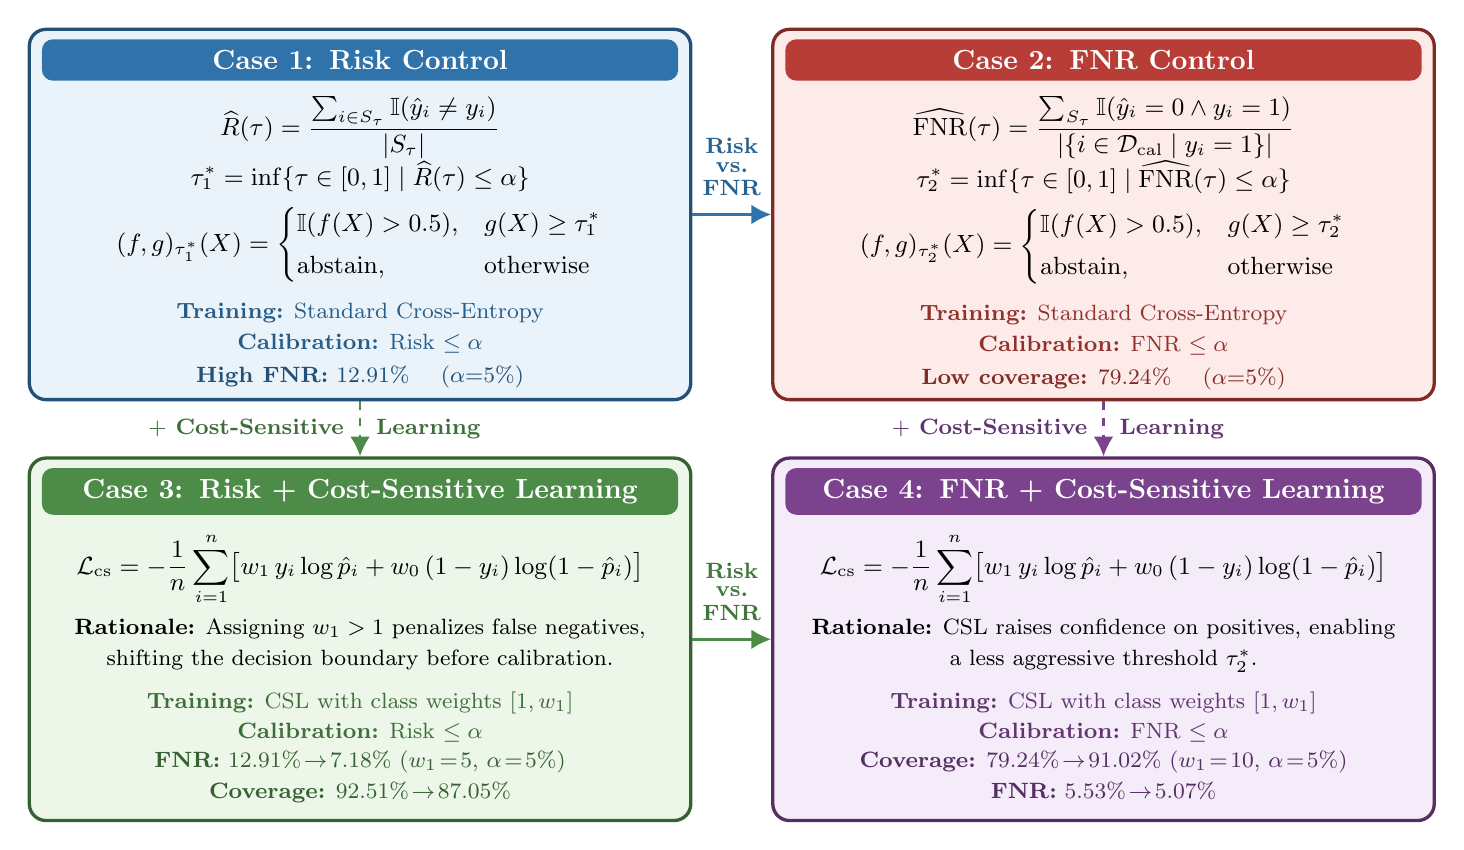
\begin{tikzpicture}[
    font=\small,
    cbox/.style n args={2}{
        rectangle, rounded corners=6pt, draw=#1!70!black, fill=#2,
        minimum width=8.4cm, 
        inner sep=10pt, line width=1.2pt
    },
    tag/.style n args={1}{
        rectangle, rounded corners=4pt, fill=#1, text=white,
        font=\bfseries, align=center, inner sep=4pt,
        text width=7.8cm, anchor=north
    },
    harrow/.style={
        -{Latex[length=2.5mm,width=2.5mm]}, line width=1pt, #1
    },
    varrow/.style={
        -{Latex[length=2.5mm,width=2.5mm]}, line width=1pt, dashed, #1
    },
]

\definecolor{c1}{RGB}{48,115,170}
\definecolor{c1bg}{RGB}{235,243,250}
\definecolor{c2}{RGB}{183,61,54}
\definecolor{c2bg}{RGB}{252,235,233}
\definecolor{c3}{RGB}{77,139,72}
\definecolor{c3bg}{RGB}{236,246,233}
\definecolor{c4}{RGB}{123,66,142}
\definecolor{c4bg}{RGB}{245,236,249}

% ============================================================
% Row 1
% ============================================================

\node[cbox={c1}{c1bg}] (c1) {
    % 高度放宽到 4.2cm，给底部留出呼吸空间
    \begin{minipage}[t][4.0cm][t]{7.6cm}\centering
    \vspace*{0.5cm}
    $\displaystyle\widehat{R}(\tau)=\frac{\sum_{i\in S_\tau}\mathbb{I}(\hat{y}_i\neq y_i)}{|S_\tau|}$
    \hspace{4pt}
    $\tau_1^*=\inf\{\tau\in[0,1]\mid\widehat{R}(\tau)\leq\alpha\}$

    \vspace{4pt} 
    $(f,g)_{\tau_1^*}(X)=
    \begin{cases}
    \mathbb{I}(f(X)>0.5), & g(X)\geq\tau_1^*\\[2pt]
    \text{abstain},       & \text{otherwise}
    \end{cases}$

    \vspace{6pt} 
    {\footnotesize\color{c1!80!black}
    \textbf{Training:} Standard Cross-Entropy \\
    \textbf{Calibration:} Risk $\leq\alpha$}\\[1pt]
    {\footnotesize\color{c1!70!black}
    \textbf{High FNR:} 12.91\% \quad ($\alpha$=5\%)}
    \end{minipage}
};
\node[tag={c1}] at ([yshift=-4pt]c1.north) {Case 1: Risk Control};

\node[cbox={c2}{c2bg}, right=1.0cm of c1] (c2) {
    % 保持左右高度一致
    \begin{minipage}[t][4.0cm][t]{7.6cm}\centering
    \vspace*{0.5cm} 
    $\displaystyle\widehat{\mathrm{FNR}}(\tau)=\frac{\sum_{S_\tau}\mathbb{I}(\hat{y}_i=0\wedge y_i=1)}{|\{i\in\mathcal{D}_{\mathrm{cal}}\mid y_i=1\}|}$
    \hspace{4pt}
    $\tau_2^*=\inf\{\tau\in[0,1]\mid\widehat{\mathrm{FNR}}(\tau)\leq\alpha\}$

    \vspace{4pt}
    $(f,g)_{\tau_2^*}(X)=
    \begin{cases}
    \mathbb{I}(f(X)>0.5), & g(X)\geq\tau_2^*\\[2pt]
    \text{abstain},       & \text{otherwise}
    \end{cases}$

    \vspace{6pt}
    {\footnotesize\color{c2!80!black}
    \textbf{Training:} Standard Cross-Entropy \\
    \textbf{Calibration:} FNR $\leq\alpha$}\\[1pt]
    {\footnotesize\color{c2!70!black}
    \textbf{Low coverage:} 79.24\% \quad ($\alpha$=5\%)}
    \end{minipage}
};
\node[tag={c2}] at ([yshift=-4pt]c2.north) {Case 2: FNR Control};

\draw[harrow={c1}]
    (c1.east) -- (c2.west)
    node[midway, above=3pt, font=\footnotesize\bfseries, text=c1!85!black, align=center]
    {\shortstack{Risk\\vs.\\FNR}};

% ============================================================
% Row 2
% ============================================================

\node[cbox={c3}{c3bg}, below=0.7cm of c1] (c3) {
    % 高度放宽到 3.9cm，防止文字溢出
    \begin{minipage}[t][3.9cm][t]{7.6cm}\centering
    \vspace*{0.6cm} 

    $\displaystyle\mathcal{L}_{\mathrm{cs}}=-\frac{1}{n}\sum_{i=1}^{n}
    \bigl[w_1\,y_i\log\hat{p}_i+w_0\,(1-y_i)\log(1-\hat{p}_i)\bigr]$

    \vspace{4pt} 
    {\footnotesize \textbf{Rationale:} Assigning $w_1>1$ penalizes false negatives, shifting the decision boundary before calibration.}

    \vspace{6pt}
    {\footnotesize\color{c3!80!black}
    \textbf{Training:} CSL with class weights $[1,w_1]$ \\
    \textbf{Calibration:} Risk $\leq\alpha$}\\[1pt]
    {\footnotesize\color{c3!70!black}
    \textbf{FNR:} $12.91\%\!\to\!7.18\%$ ($w_1\!=\!5$, $\alpha\!=\!5\%$) \\
    \textbf{Coverage:} $92.51\%\!\to\!87.05\%$}
    \end{minipage}
};
\node[tag={c3}] at ([yshift=-4pt]c3.north) {Case 3: Risk + Cost-Sensitive Learning};

\node[cbox={c4}{c4bg}, right=1.0cm of c3] (c4) {
    % 保持左右高度一致
    \begin{minipage}[t][3.9cm][t]{7.6cm}\centering
    \vspace*{0.6cm}

    $\displaystyle\mathcal{L}_{\mathrm{cs}}=-\frac{1}{n}\sum_{i=1}^{n}
    \bigl[w_1\,y_i\log\hat{p}_i+w_0\,(1-y_i)\log(1-\hat{p}_i)\bigr]$

    \vspace{4pt}
    {\footnotesize \textbf{Rationale:} CSL raises confidence on positives, enabling a less aggressive threshold $\tau_2^*$.}

    \vspace{6pt}
    {\footnotesize\color{c4!80!black}
    \textbf{Training:} CSL with class weights $[1,w_1]$ \\
    \textbf{Calibration:} FNR $\leq\alpha$}\\[1pt]
    {\footnotesize\color{c4!70!black}
    \textbf{Coverage:} $79.24\%\!\to\!91.02\%$ ($w_1\!=\!10$, $\alpha\!=\!5\%$) \\
    \textbf{FNR:} $5.53\%\!\to\!5.07\%$}
    \end{minipage}
};
\node[tag={c4}] at ([yshift=-4pt]c4.north) {Case 4: FNR + Cost-Sensitive Learning};

\draw[harrow={c3}]
    (c3.east) -- (c4.west)
    node[midway, above=3pt, font=\footnotesize\bfseries, text=c3!85!black, align=center]
    {\shortstack{Risk\\vs.\\FNR}};

% Vertical arrows (使用 \strut 保证左右两段文字基线绝对对齐)
\draw[varrow={c3}]
    (c1.south) -- 
    node[midway, left=2pt, font=\footnotesize\bfseries, text=c3!80!black] {$+$ Cost-Sensitive\strut}
    node[midway, right=2pt, font=\footnotesize\bfseries, text=c3!80!black] {Learning\strut}
    (c3.north);

\draw[varrow={c4}]
    (c2.south) -- 
    node[midway, left=2pt, font=\footnotesize\bfseries, text=c4!80!black] {$+$ Cost-Sensitive\strut}
    node[midway, right=2pt, font=\footnotesize\bfseries, text=c4!80!black] {Learning\strut}
    (c4.north);

\end{tikzpicture}
\end{document}